\newpage
\section{DMA (Direct Memory Access)}\label{par:DMA}
Il \textbf{DMA (Direct Memory Access)} è un dispositivo che permette di sollevare il processore dall'onere di trasferire i dati tra varie periferiche. Per precisare meglio tale concetto, il DMA permette di gestire il trasferimento dati tra:
\begin{itemize}
    \item \textbf{Memoria-Periferica}
    \item \textbf{Periferica-Memoria}
    \item \textbf{Memoria-Memroia}
\end{itemize}

Il suo principio di funzionamento è semplice, ed è schematizzabile su 3 registri principali, dove principalmente si vanno a specificare:
\begin{itemize}
    \item \textbf{Registro Indirizzo}: Indica l'indirizzo da cui prelevare il dato
    \item \textbf{Registro Conteggio}: Indica il conteggio del numero di "dati" trasferiti, e permette di capire quando bisogna interrompere il trasferimento
    \item \textbf{Registro Identificativo}: Tramite tale registro si vanno ad identificare, o il dispositivo da considerare o l'area di memoria in cui andare a trasferire i dati
\end{itemize}

La reale architettura del DMA è però ben diversa, essa risulterà più complicata. La maggior complessità dell'architettura proviene da varie tipologie di problematiche che si possono riscontrare all'interno del suo utilizzo, come, ad esempio, l'accesso al BUS dati in maniera concorrente rispetto al processore. \uppercase{è} pertanto necessario che il DMA non sia collegato al processore solo tramite il bus dato, ma anche tramite vari bus di controllo, che permettono al processore ed al DMA di poter comunicare in base ai vari accessi in memoria ecc.

Il dispositivo a cui si andrà a fare riferimento nelle nostre esercitazioni sarà l'Intel 8237, che per la sua architettura ha 4 canali distinti (quindi è in grado di gestire 4 trasferimenti alla volta). Nella sua versione in ASIM, tale componente è composto di soli 2 canali, quindi è un sua versione semplificata.
Scendendo più nei dettagli, tale dispositivo è in grado di sostenere 4 modalità di funzionamento differenti, ovvero:
\begin{itemize}
    \item \textbf{Single}: Ad ogni ciclo, si ferma e lascia altri cicli per il processore. Ricomincia a trasmettere quando la linea di richiesta sarà di nuovo attiva
    \item \textbf{Block}: La linea di richiesta viene controllata una singola volta, una volta attivato il trasferimento, il BUS, sarà rilasciato solo dopo aver finito il trasferimento
    \item \textbf{Demand}: Simile alla modalità Block, con l'unica differenza che il trasferimento prosegue fin tanto che la richiesta è attiva, se dovesse fermarsi, attende, e quando ricomincia, riprende da dove aveva lasciato (non si resetta)
    \item \textbf{Cascade}: Modalità di funzionamento che permette di collegare più DMA in cascata in modo da poter avere dispositivi con più di 4 canali
\end{itemize}

Oltre al minor numero di canali, il componente simulato in ASIM non supporta tutte le modalità sopra-citate, difatti le modalità utilizzabili in ASIM sono:
\begin{itemize}
    \item \textbf{Single}
    \item \textbf{Block}
\end{itemize}

Guardando la figura [\ref{img:DMA}], abbiamo il modello architetturale del componente realizzato in ASIM, di cui i registri posti sulla sinistra sono di comunicazione con il processore, mentre i segnali sulla destra sono quelli che vengono utilizzati per l'interfacciamento con le periferiche collegate ai corrispettivi canali.

Per la comunicazione con il processore, il significato che hanno i segnali rappresentati è il seguente:
\begin{itemize}
    \item \textbf{D0-D7}: collegamento al BUS dati da e verso il componente
    \item \textbf{CS}: segnale binario di selezione del dispositivo
    \item \textbf{A0-A3}: Attenzione non tutti i segnali A, ma solo i 4 meno significativi, vengono utilizzati per la selezione dello specifico registro interno da considerare
    \item \textbf{IOR e IOW}: Segnali di gestione della lettura e della scrittura sul componente e per le periferiche
    \item \textbf{MEMR e MEMW}: Segnali di gestione della lettura e della scrittura sui dispositivi di memoria
    \item \textbf{CLK e Reset}: Classici segnali di clock (tempificazione delle operazioni) e reset (si vanno a cancellare tutti i registri del dispositivo)
    \item \textbf{HRQ}: Segnale di richiesta del controllo del sistema BUS, che solitamente è collegata all'ingresso HOLD della CPU
    \item \textbf{HLDA}: Segnale proveniente dalla CPU che segnala l'acquisizione del sistema BUS da parte del processore
    \item  \textbf{EOP}: Linea di interruzione che bisogna collegare al processore per segnalare il completamento del trasferimento richiesto
\end{itemize}

Dati i due differenti canali si avranno 2 periferiche collegate allo stesso dispositivo DMA. Pertanto, la comunicazione, potrà essere effetuata da una sola di queste periferiche per volta. Tale decisione viene effettuata secondo un ordine di priorità, per cui il dispositivo collegato ai terminali 0 avrà una priorità maggiore rispetto a quello collegato ai terminali 1. I segnali che gestiscono le periferiche sono:
\begin{itemize}
    \item \textbf{DREQ 0 e DREQ 1}: Che sono due segnali che utilizzano le periferiche per richiedere l'accesso al BUS tramite dei cicli DMA
    \item \textbf{DACK 0 e DACK 1}; Sono due segnali che permettono di comunicare alla periferica (da parte del DMA), che sono abilitate per un determinato ciclo DMA
\end{itemize}

\begin{figure}
    \centering
    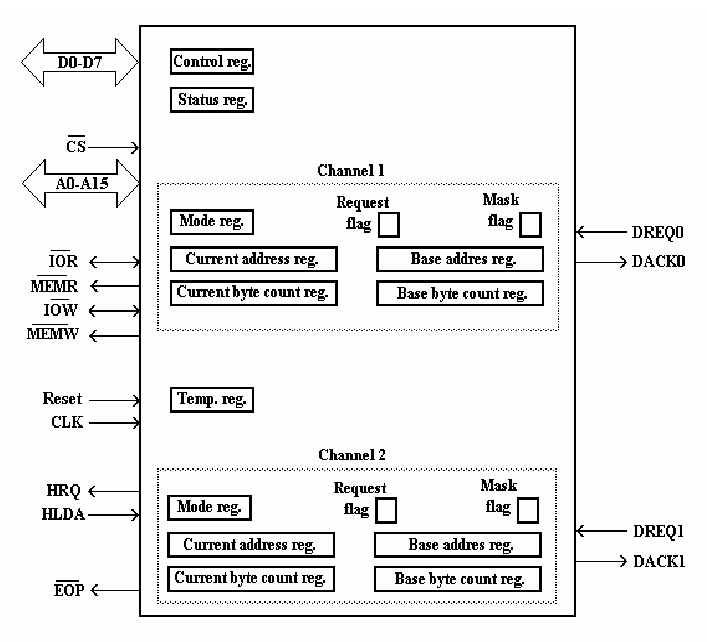
\includegraphics[width=.7\textwidth]{img/DMA.png}
    \caption{DMA a 2 canali}\label{img:DMA}
\end{figure}


